\section{Towards the Te-loaded Phase}

\subsection{Muon Induced Backgrounds in the Te-loaded Phase}
This analysis is aimed to estimate the background isotopes created by the muon interacting on the $^{12}$C atoms in the liquid scintillator.

\begin{table}[ht]
	%%%%\footnotesize
	\caption{Cosmic muon induced isotopes production rates $R_i~[kt^{-1}yr^{−1}]$. Taken from \cite{nndc}.}\label{estimateRates}
	\centering
	\scriptsize
	\begin{tabular*}{170mm}{c@{\extracolsep{\fill}}cccccccc}
		\toprule 
		\multirow{2}{*}{isotopes} &\multicolumn{2}{c}{NA54 mean}& NA54 distr.& \multicolumn{2}{c}{KamLAND}& \multicolumn{2}{c}{Borexino}\\
		\cline{2-3}   \cline{5-6} \cline{7-8}
		& solar & Te & solar  & solar & Te & solar & Te\\
		\midrule
		$^{11}$C &559.72$\pm$55.81 &524.34$\pm$52.28 &190$\pm$33 &1135.1$\pm$206.21 &1063.34$\pm$193.17& 1048$\pm$121 &981.75$\pm$113.35\\
		$^{12}$B & -- & -- & -- & 59.94$\pm$5.41& 56.15$\pm$5.07 &69$\pm$3 &65$\pm$3\\
		$^{11}Be$&  1.45$\pm$0.11& 1.36$\pm$0.10& -- &1.50$\pm$0.35 &1.41$\pm$0.33& $<8.5$ & $<7.96$ \\
                $^{11}Li$ & -- & -- & -- & -- & -- & -- & --\\
		$^8$Li & 2.49$\pm$0.92 & 2.33$\pm$0.86 & 1$\pm$1 & 15.64$\pm$3.47 & 14.65$\pm$2.35 & 8$\pm$7 & 7$\pm$7\\
		$^8$He ($^8$He+$^9$Li) & 1.31$\pm$0.24 & 1.23$\pm$0.22 & -- & 1.13$\pm$0.57 & 1.05$\pm$0.53 & $<1.9$ & $<1.8$\\
		$^9$Li & --&  --&  --&  3.04$\pm$0.34 & 2.85$\pm$0.32 & 3.6$\pm$0.3 & 3.4$\pm$0.3\\
        $^6$He & 9.91$\pm$1.25 & 9.28$\pm$1.17 & 3$\pm$1 &-- &-- &46$\pm$16 & 43$\pm$15\\
		$^{10}$C & 71.37$\pm$10.55 & 66.86$\pm$9.88 & 24$\pm$6 & 22.63$\pm$2.73 & 21.20$\pm$2.56 & 22$\pm$5 & 21$\pm$5\\
        $^9$C & 2.99$\pm$0.96 & 2.80$\pm$0.90 & -- & 4.09$\pm$1.65 & 3.83$\pm$1.55 & $<19.3$ & $<18.1$\\
        $^8$B & 4.41$\pm$0.96 & 4.13$\pm$0.90 & 2$\pm$1 & 10.05$\pm$2.86 & 9.41$\pm$2.68 & 16$\pm$6 & 15$\pm$6\\
		$^7$Be &142.25$\pm$17.90 & 133.26$\pm$16.77 & 55$\pm$15 & -- & -- & -- & --\\
		$^{12}$N & -- &--& --& --& --& $<1.88$ & $<1.76$\\
		\bottomrule
	\end{tabular*}
\end{table}


\begin{table}[ht]
	\caption{Decay information of the isotopes. Taken from \cite{nndc}.}\label{decayIso}
	\centering	
	\begin{tabular*}{100mm}{c@{\extracolsep{\fill}}ccc}
		\toprule 
		isotope &half-life & Q-value &  Decay mode\\
		\midrule
		$^{11}$C & 20.334 min & 0.96 MeV&  $^{11}$C$\to ^{11}$B$+e^++\nu_e$\\
		$^{10}$C & 19.308 s & 3.65 MeV & $^{10}$C$\to^{10}$B$+e^+ +\nu_e$\\
		$^{6}$He &806.7 ms & 3.51 MeV &  $^{6}$He$\to^{6}Li+e^-+\nu_e$\\
		\bottomrule	
	\end{tabular*}
\end{table}  



To simulate these backgrounds, the optics for $0.3~\%$ Te by weight and with $bisMSB$ ($te\_0p3\_labppo\_scintillator\_bisMSB\_Feb2015$)
and RAT-5.2.3 were used.



I looked into 10000 simulations of the cosmic muon induced $^{11}$C, $^{10}$C and $^6$He backgrounds events. Each simulation runs for one
year duration.

Fig.~\ref{muon_c11}, Fig.~\ref{muon_c10} and Fig.~\ref{muon_He6} show the spectrum of the Monte Carlo energies (mc Edep quenched) scaled from 10000 simulations
(left) and the scaled spectrum of the reconstructed energies (right) for one year duration and one kilo-tonne of the
cocktail. The fiducial volume (FV) cuts of 5.5-m, 4.5-m, 3.5-m are applied.

The Monte Carlo results give a total 11C background rate of 1063.55 $kt^{-1}yr^{-1}$ without cuts, 21.39 $kt^{-1}yr^{-1}$ for
$^{10}$C and 43.31 $kt^{-1}yr^{-1}$ for $^6$He.
From results of the reconstructed energies, a total background rate of 989.17 $kt^{-1}yr^{-1}$ for $^{11}$C is evaluated while
20.06 $kt^{-1}yr^{-1}$ for $^{10}$C and 40.07 $kt^{-1}yr^{-1}$ for $^6$He.

For the region of interest (ROI) of the $^{130}$Te $0\nu\beta\beta$ search, we defined the ROI windows by simulating 10000 events of $0\nu\beta\beta$,
fitting the $0\nu\beta\beta$ signal peak with Gaussian function and taking the -0.5$\sigma$ to 1.5$\sigma$ region around the Gaussian signal
peak. The ROI window of $[2.47, 2.70]~MeV$ taken from \cite{whitepaper} is also checked. From both
results of the Monte Carlo and reconstruction, after the 5.5-m FV cut, no events of $^{11}$C backgrounds in the ROI are
expected; after the 3.5-m FV cut, the event rates of $^{10}$C and $^6$He are below 1 $kt^{-1}yr^{-1}$ in the ROI. Among these
three backgrounds, the $^{10}$C has the highest event rates in the ROIs.
The event rates for these three isotopes backgrounds with different FV cuts and different ROI windows are
summarized in Table.~\ref{muon_eventrates}. The values obtained from the Monte Carlo simulations are listed in the ``MC" column and
from the reconstruction are listed in the ``Recon" column.

\begin{table}[ht]
	\caption{Production rates for $^{11}$C, $^{10}$C and $^{6}$He backgrounds in SNO+ Te-loaded Phase.}\label{productionRates}
				\centering	
	\begin{tabular*}{100mm}{c@{\extracolsep{\fill}}ccc}
			\toprule 
			isotope & rates [$kt^{-1}\cdot yr^{-1}$]& rates [Hz]\\
			\midrule
		 $^{11}$C & 1063.34 & 0.00003372\\
		 $^{10}$C & 21.20 & 0.0000006722\\
		 $^{6}$He &43.09& 0.0000013663 \\
			\bottomrule	
	\end{tabular*}
\end{table}

\begin{figure}[htbp]
	\subfigure{
		\begin{minipage}[t]{0.45\textwidth}
			\centering
			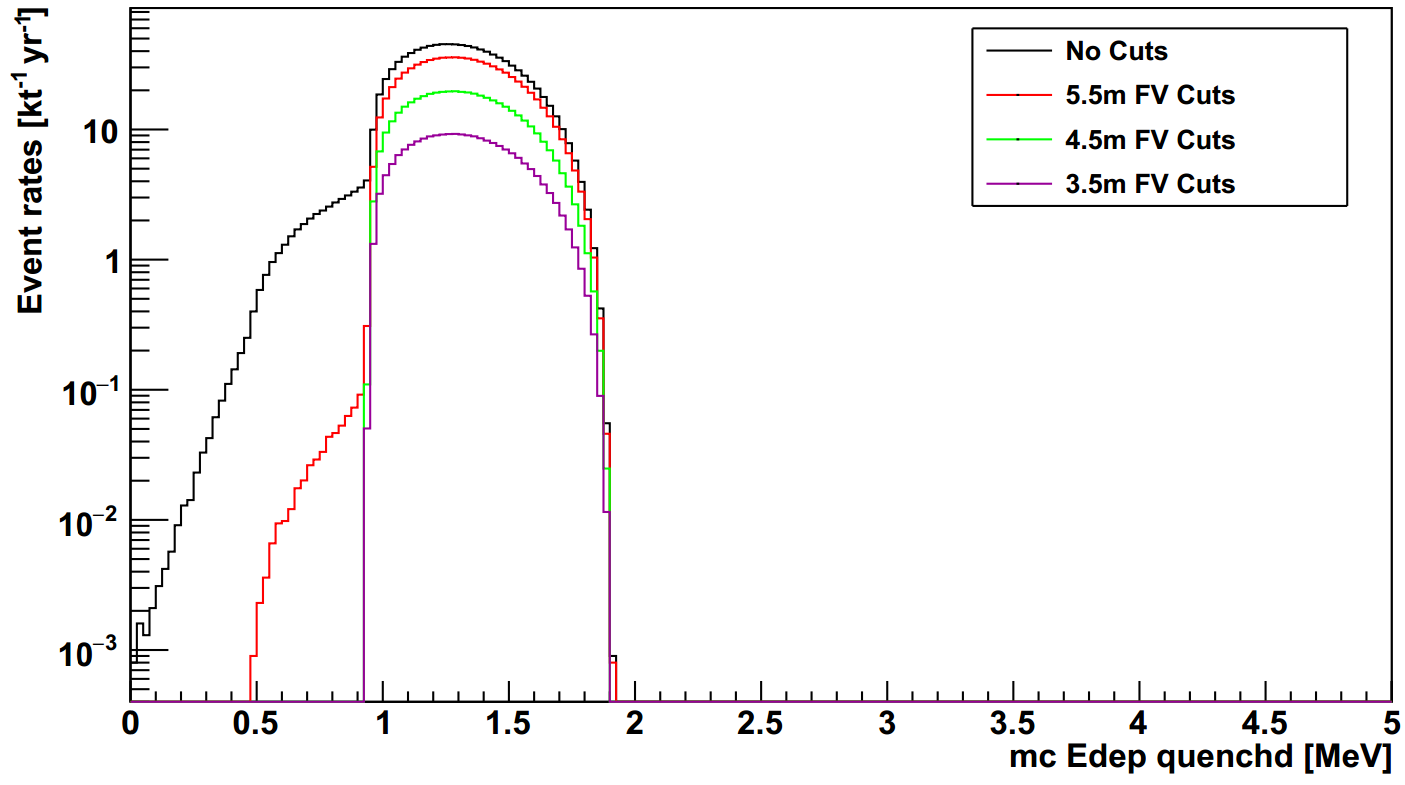
\includegraphics[width=7cm]{muon_mcC11.png}
		\end{minipage}
	}   
	\subfigure{ 
		\begin{minipage}[b]{0.3\textwidth}
			\centering
			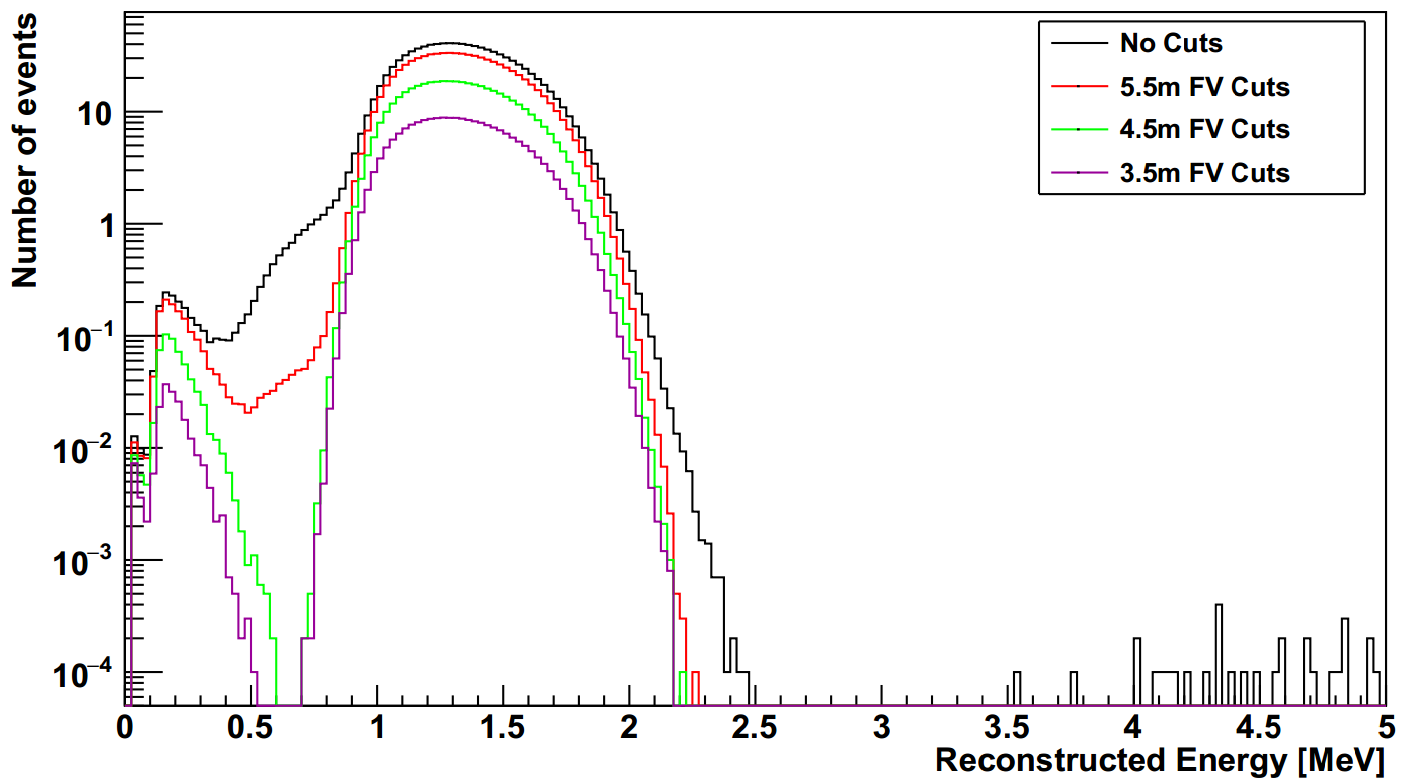
\includegraphics[width=7cm]{muon_reconC11.png}
		\end{minipage}
	}
	\caption{Energy spectrum of cosmic muon induced $^{11}$C backgrounds in SNO+ Te-loaded phase for one year duration. Left: Monte Carlo energy distributions. Right: Reconstructed energy distributions.}
	\label{muon_c11}
\end{figure}

\begin{figure}[htbp]
	\subfigure{
		\begin{minipage}[t]{0.45\textwidth}
			\centering
			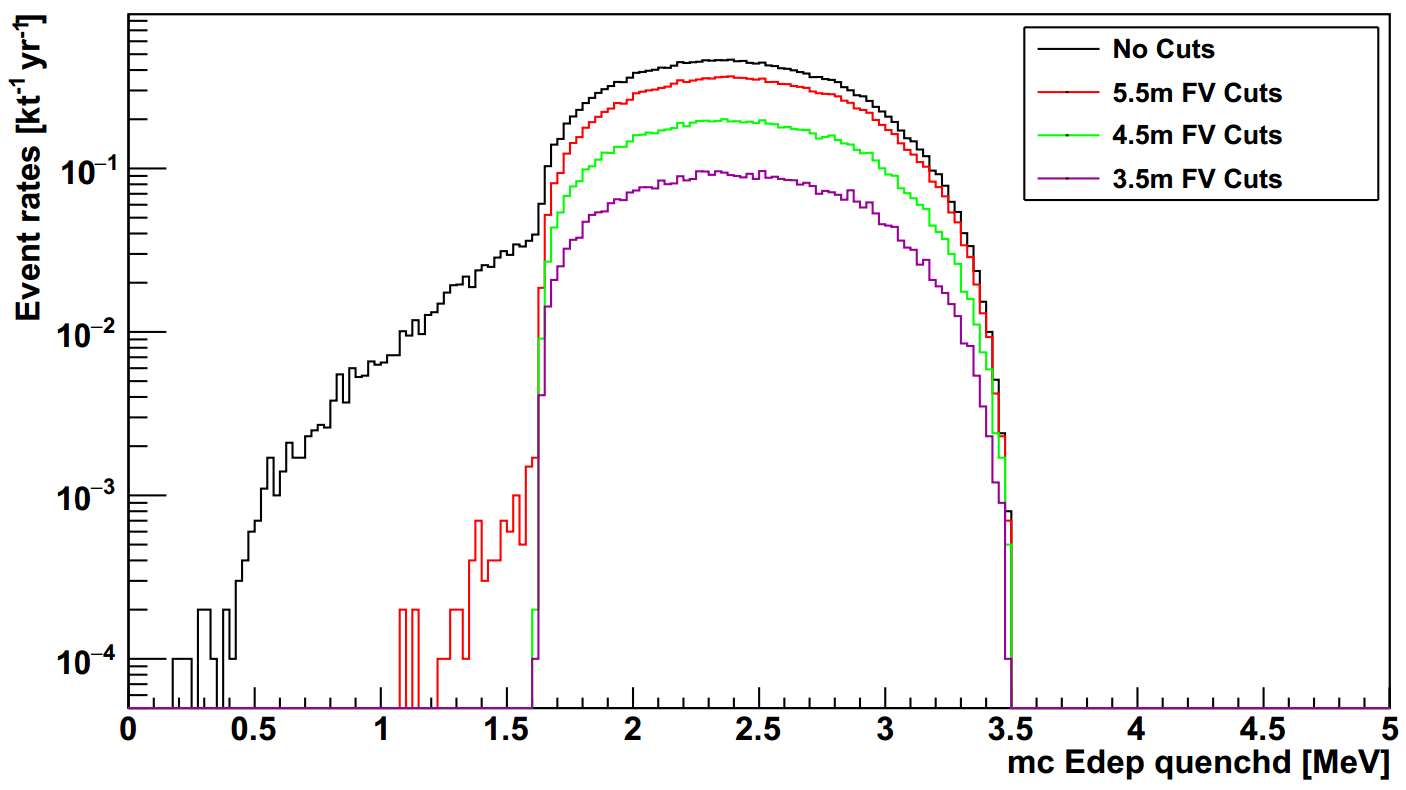
\includegraphics[width=6.5cm]{muon_mcC10.png}
		\end{minipage}
	}   
	\subfigure{ 
		\begin{minipage}[b]{0.3\textwidth}
			\centering
			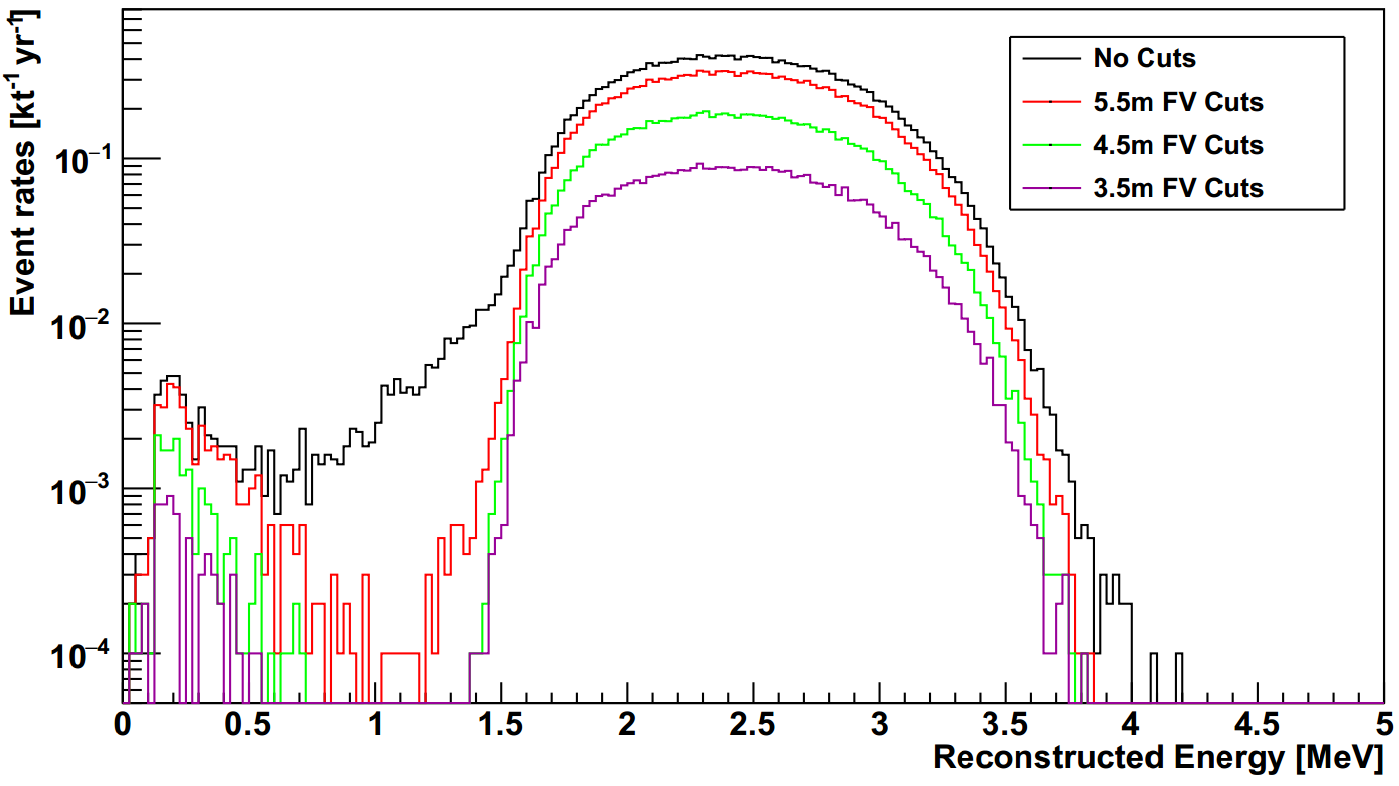
\includegraphics[width=6.5cm]{muon_reconC10.png}
		\end{minipage}
	}
	\caption{Energy spectrum of cosmic muon induced $^{10}$C backgrounds in SNO+ Te-loaded phase for one year duration. Left: Monte Carlo energy distributions. Right: Reconstructed energy distributions.}
	\label{muon_c10}
\end{figure}

\begin{figure}[htbp]
	\subfigure{
		\begin{minipage}[t]{0.45\textwidth}
			\centering
			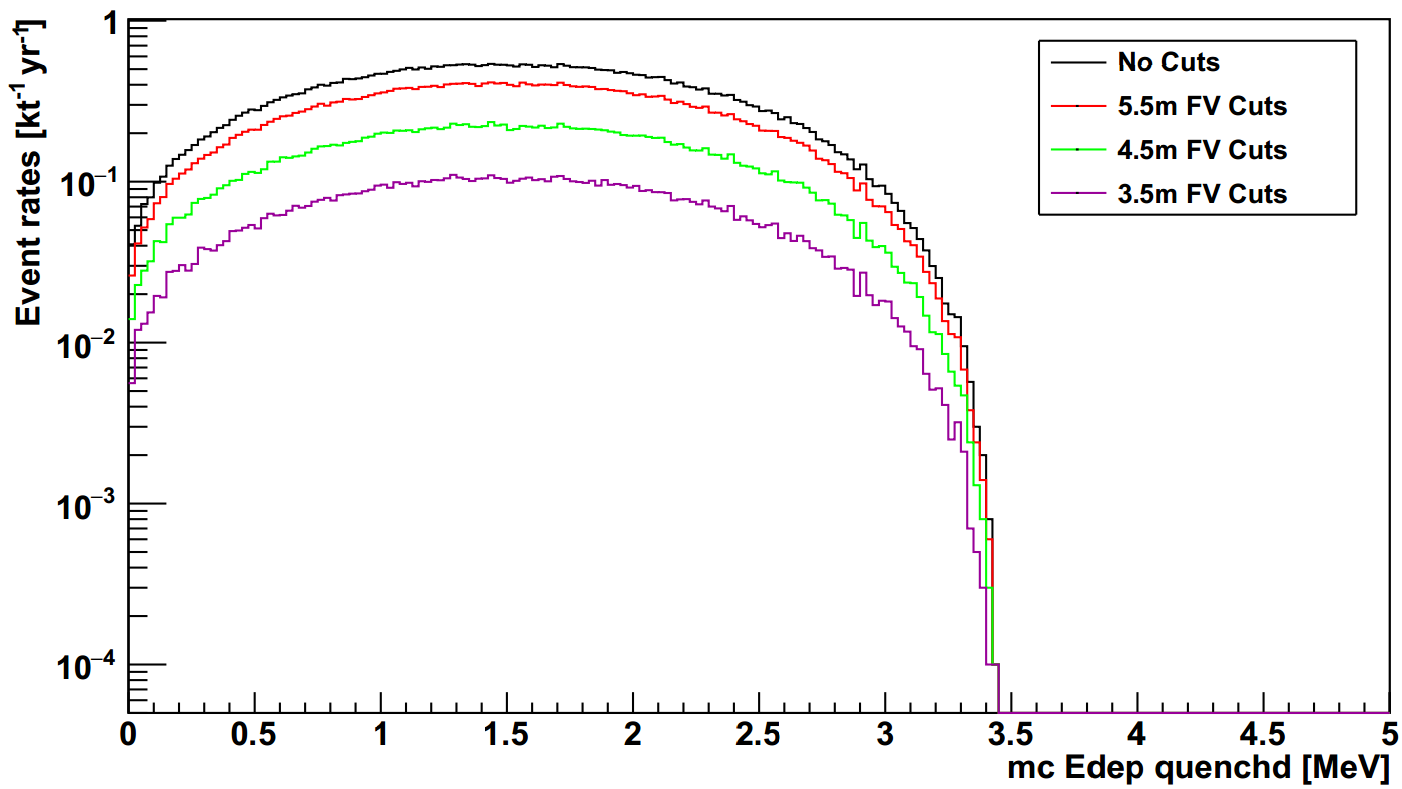
\includegraphics[width=6.5cm]{muon_mcHe6.png}
		\end{minipage}
	}   
	\subfigure{ 
		\begin{minipage}[b]{0.3\textwidth}
			\centering
			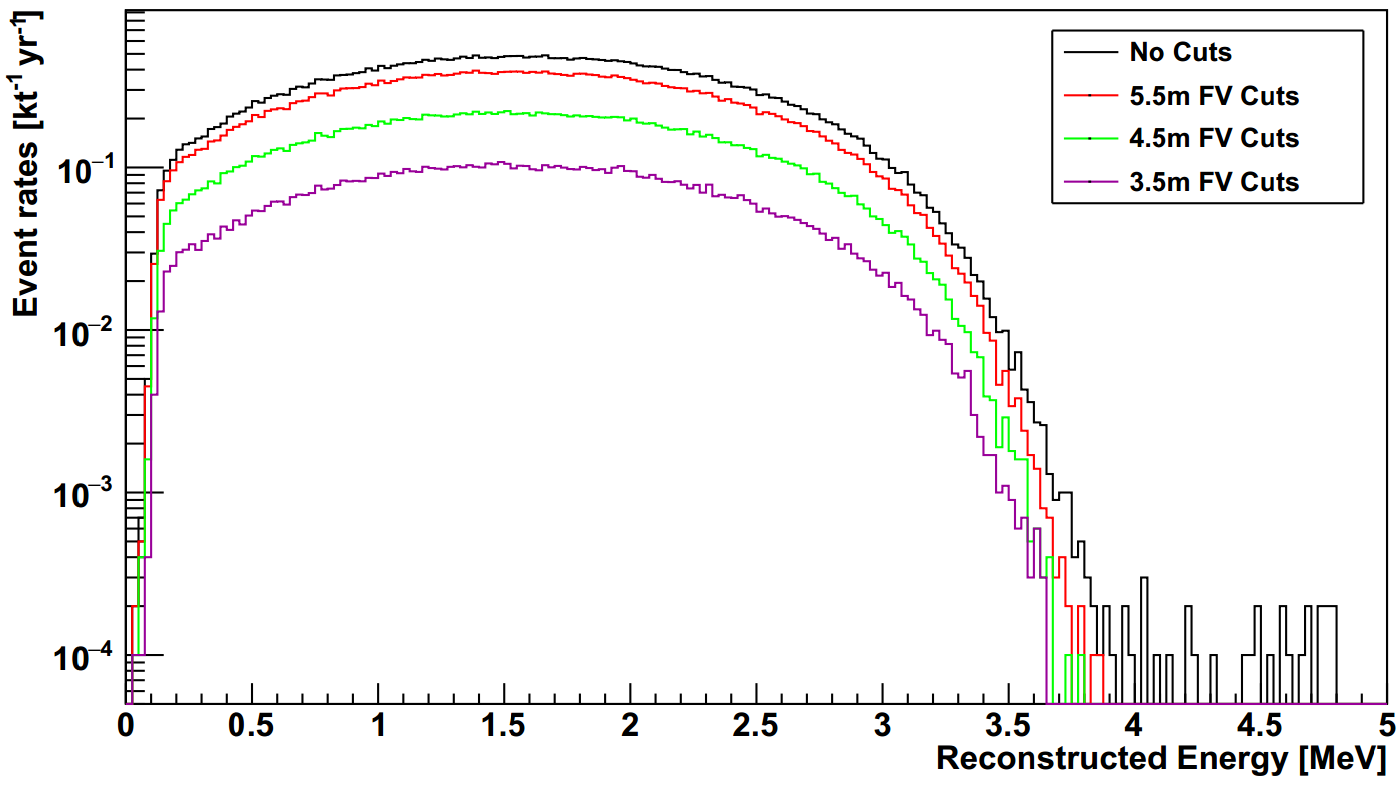
\includegraphics[width=6.5cm]{muon_reconHe6.png}
		\end{minipage}
	}
	\caption{Energy spectrum of cosmic muon induced $^{6}$He backgrounds in SNO+ Te-loaded phase for one year duration. Left: Monte Carlo energy distributions. Right: Reconstructed energy distributions.}
	\label{muon_He6}
\end{figure}

\begin{table}[ht]
	\caption{Event rates of cosmic muon induced $^{11}$C, $^{10}$C and $^{6}$He backgrounds in SNO+ Te-loaded Phase (unit: $kt^{-1}\cdot yr^{-1}$). 
		Different fiducial volume (FV) cuts and ROI region cuts are applied. The ``MC" Column presents the values obtained from the Monte Carlo and the ``Recon." column presents the values obtained from the reconstructed energies.}
	\centering
	\begin{tabular*}{150mm}{c@{\extracolsep{\fill}}cccccccc}
		\toprule
		\multirow{2}{*}{FV cuts} & \multirow{2}{*}{ROI [MeV]} & \multicolumn{2}{c}{$^{11}$C} & \multicolumn{2}{c}{$^{10}$C} & \multicolumn{2}{c}{$^{6}$He}\\
		\cline{3-4}  \cline{5-6} \cline{7-8}
		&  & MC&Recon. &MC&Recon.& MC&Recon.\\
		\midrule
		No cuts & all regions& 1063.55& 989.17 &21.39 &20.06& 43.31& 40.07\\	
		&[2.47, 2.70] &0 &1& 4.52& 4.31 &2.78& 2.88\\
		&[2.492, 2.737] &0& 0& 4.44& 4.25& 2.67& 2.79\\
		5.5-m & all regions & 807.06& 786.81& 16.24& 15.72& 32.92& 32.04\\
		&[2.47, 2.70] &0 &0 &3.63 &3.45 &2.13 &2.25\\
		&[2.487, 2.711] &0 &0 &3.28 &3.12 &1.90 &2.00\\
		4.5-m & all regions & 442.00 &437.00 &8.87 &8.72 &18.04 &17.83\\
		&[2.47, 2.70]& 0 &0& 2.00& 1.92& 1.16& 1.23\\
		&[2.477, 2.692]& 0& 0& 1.64 &1.57& 0.95& 1.01\\
		3.5-m & all regions & 207.84& 206.34& 4.20& 4.16& 8.47& 8.42\\
		&[2.47, 2.70]& 0& 0& 0.95& 0.92& 0.54& 0.57\\
		&[2.477, 2.688]& 0& 0& 0.78& 0.76& 0.44& 0.46\\
		\bottomrule		
	\end{tabular*}\label{muon_eventrates}
\end{table}

In addition, the muon-induced 11C, 10C and 6He backgrounds in the solar phase are also checked. Fig.~\ref{muonSolarC11} to Fig.~\ref{muonSolarHe6}
show the scaled spectrum from 10000 simulations of these background events in the solar phase
for 1 year duration. The total event rates are summarized in Table.~\ref{muon_eventrates2}.

\begin{figure}[htbp]
	\subfigure{
		\begin{minipage}[t]{0.45\textwidth}
			\centering
			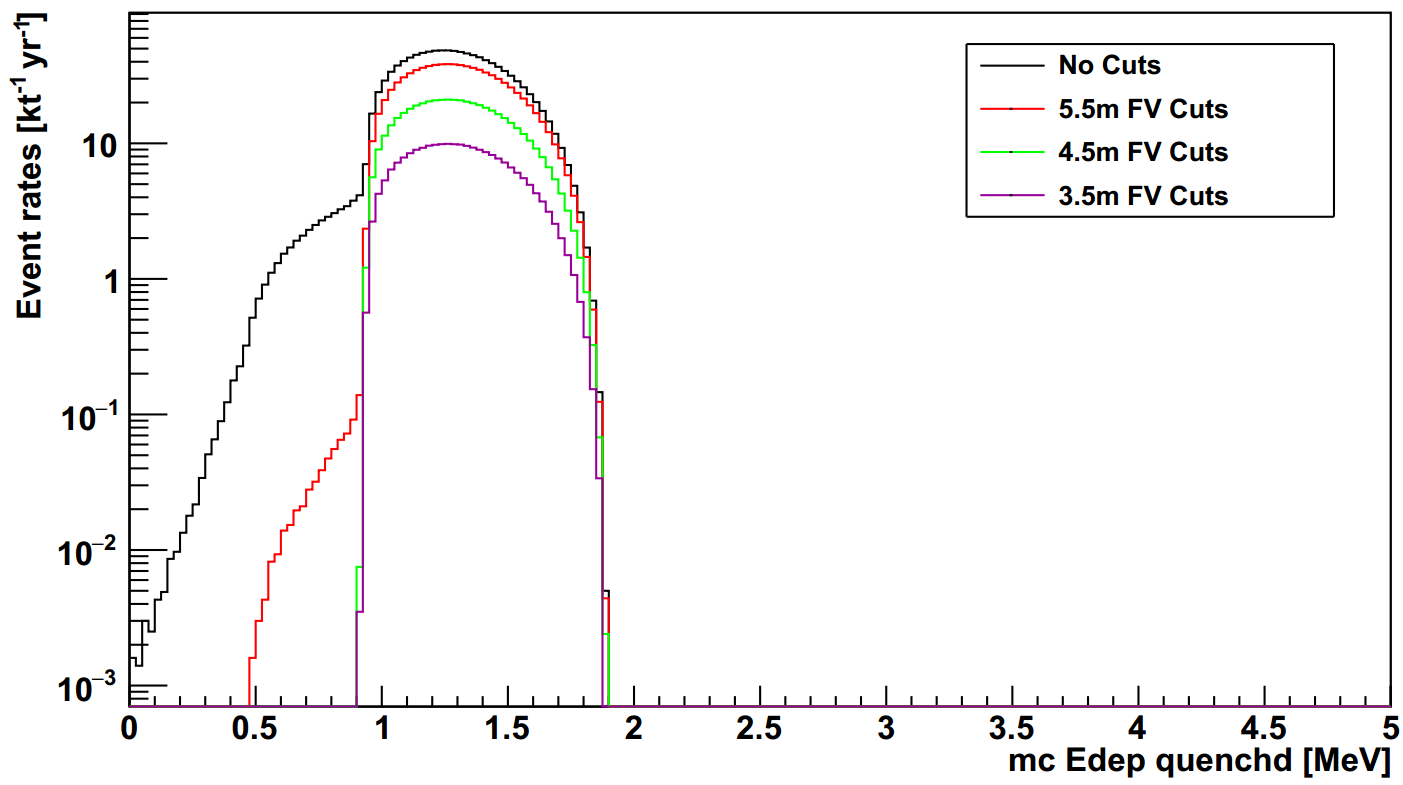
\includegraphics[width=7cm]{muonSolarMcC11.png}
		\end{minipage}
	}   
	\subfigure{ 
		\begin{minipage}[b]{0.3\textwidth}
			\centering
			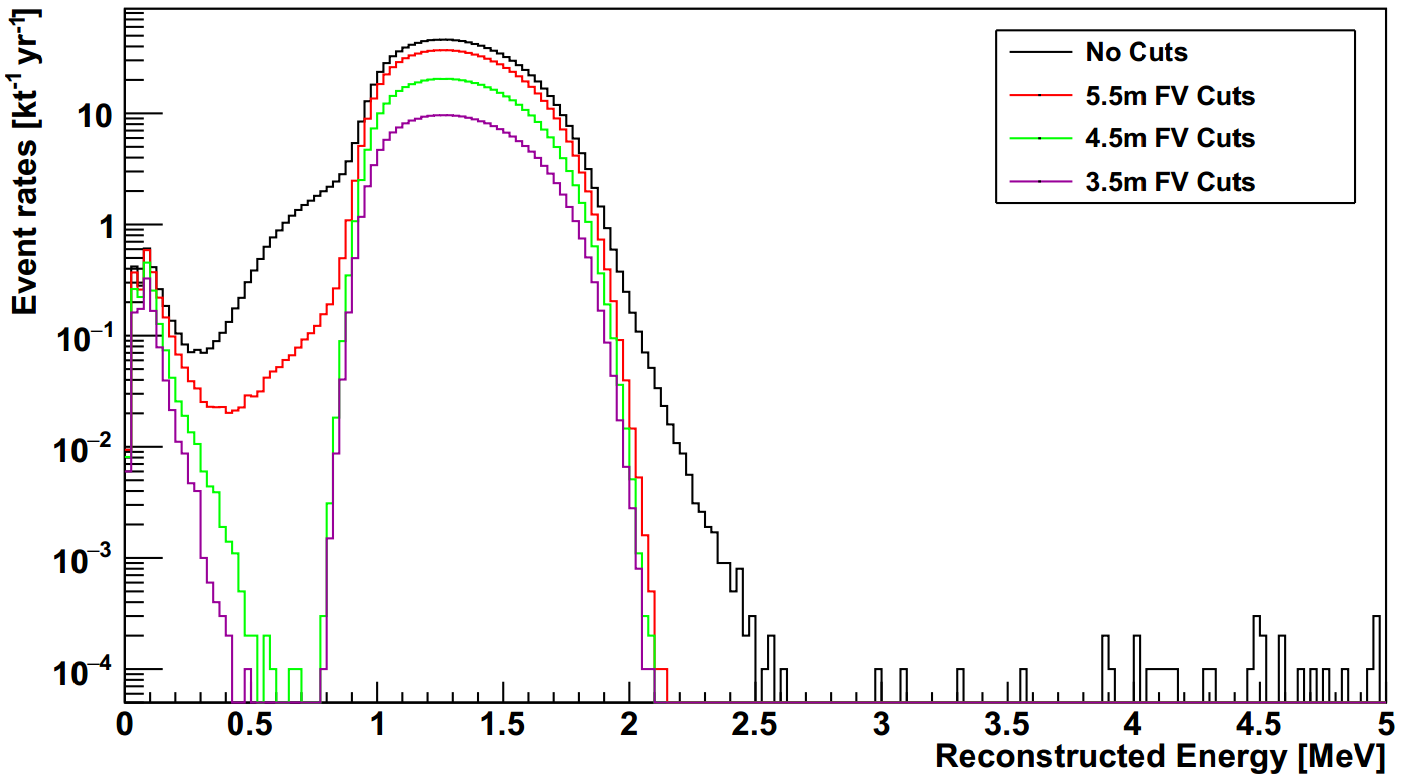
\includegraphics[width=7cm]{muonSolarReconC11.png}
		\end{minipage}
	}
	\caption{Energy spectrum of cosmic muon induced $^{11}$C backgrounds in SNO+ solar phase for one year duration. Left: Monte Carlo energy distributions. Right: Reconstructed energy distributions.}
	\label{muonSolarC11}
\end{figure}

\begin{figure}[htbp]
	\subfigure{
		\begin{minipage}[t]{0.45\textwidth}
			\centering
			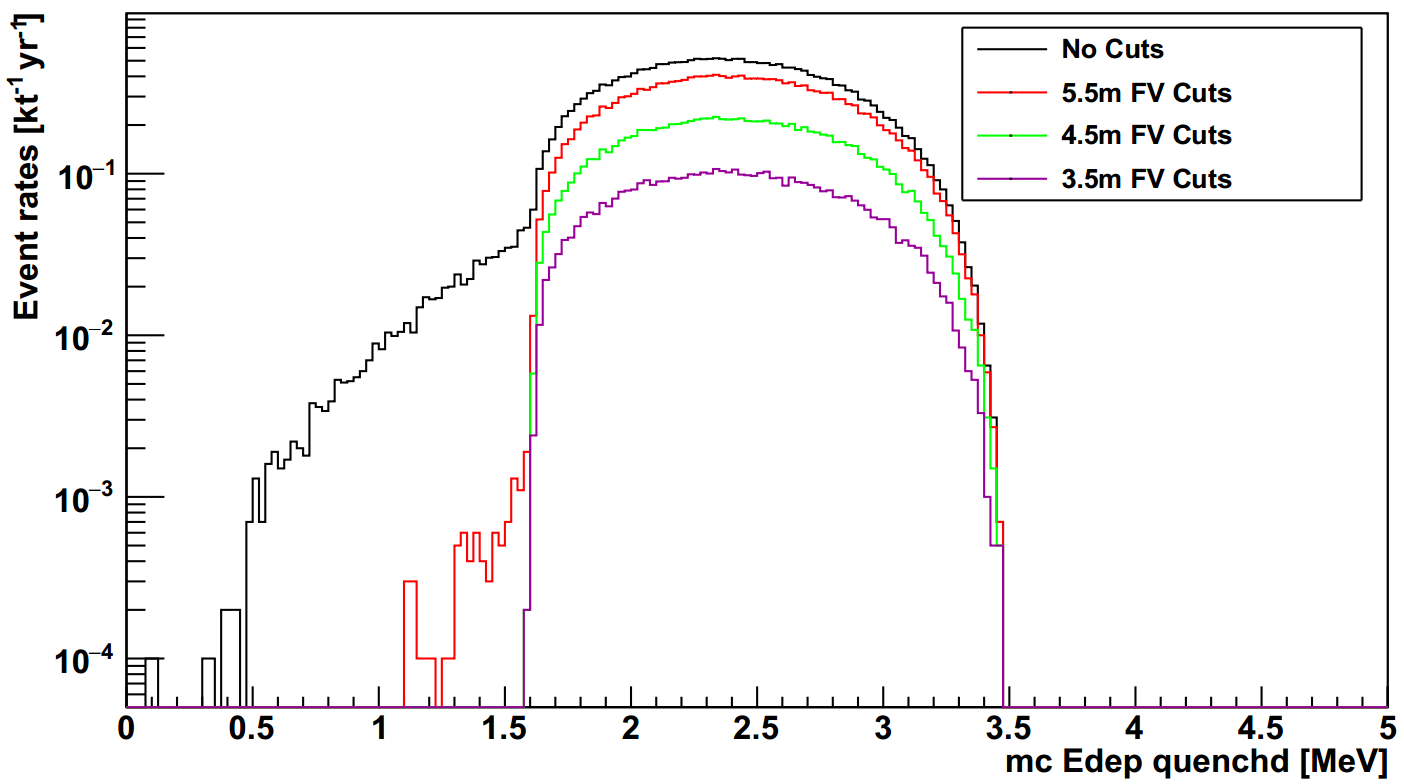
\includegraphics[width=7cm]{muonSolarMcC10.png}
		\end{minipage}
	}   
	\subfigure{ 
		\begin{minipage}[b]{0.3\textwidth}
			\centering
			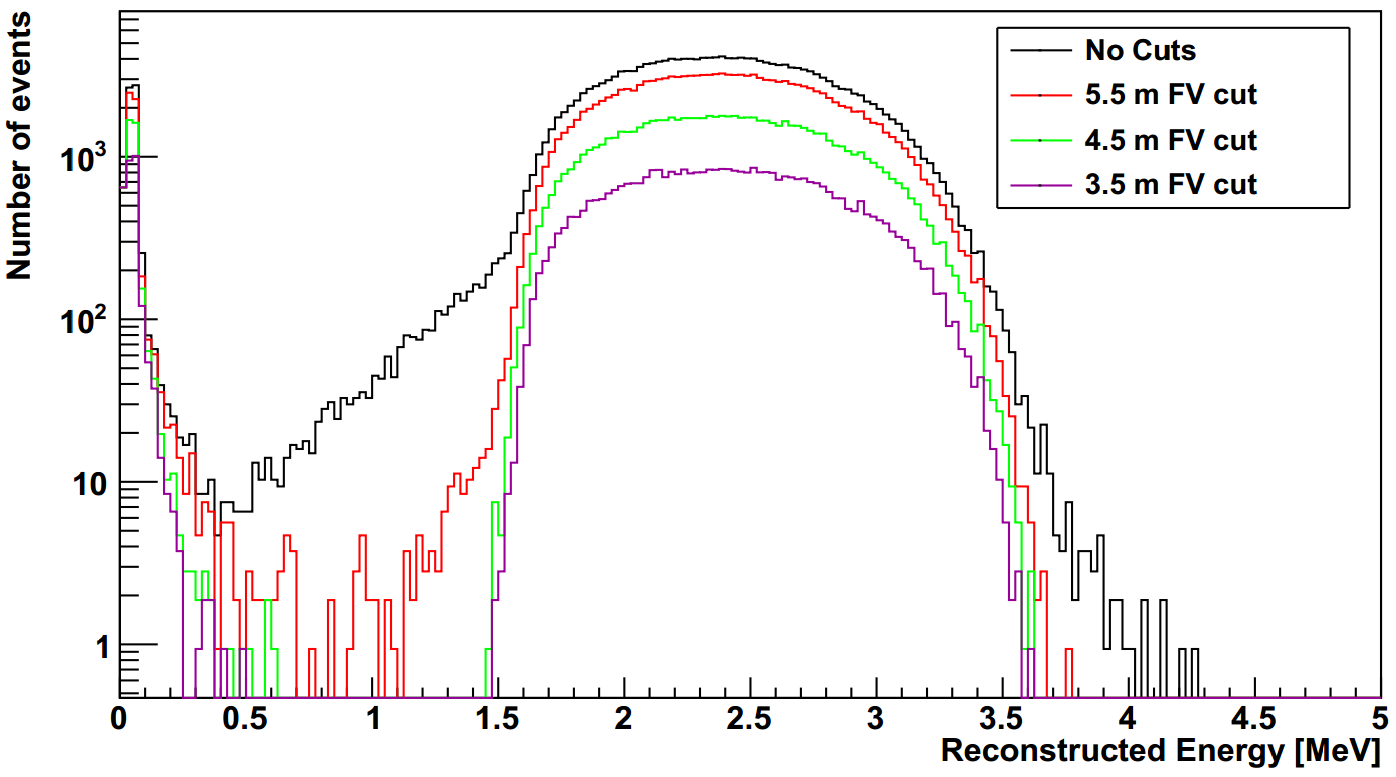
\includegraphics[width=7cm]{muonSolarReconC10.png}
		\end{minipage}
	}
	\caption{Energy spectrum of cosmic muon induced $^{10}$C backgrounds in SNO+ solar phase for one year duration. Left: Monte Carlo energy distributions. Right: Reconstructed energy distributions.}
	\label{muonSolarC10}
\end{figure}

\begin{figure}[htbp]
	\subfigure{
		\begin{minipage}[t]{0.45\textwidth}
			\centering
			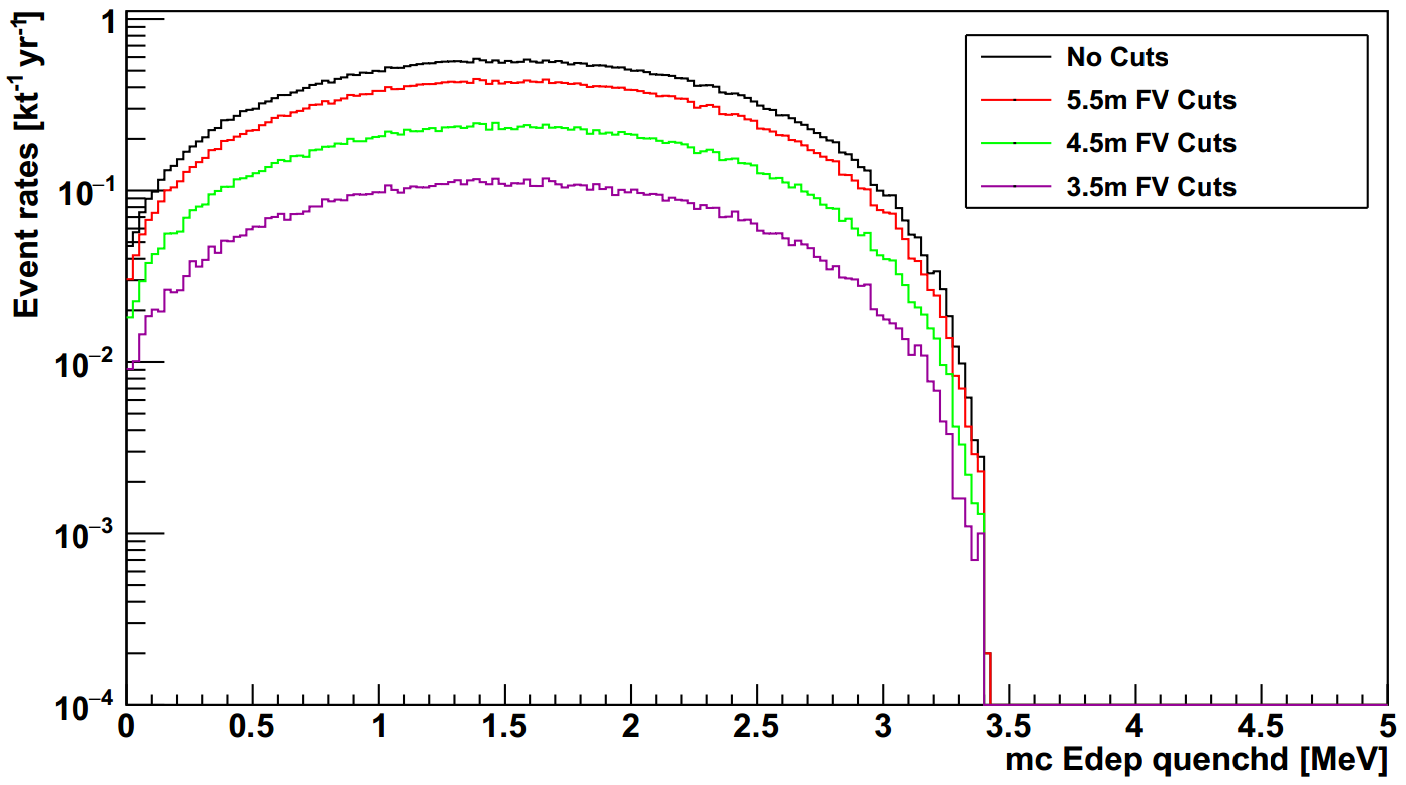
\includegraphics[width=7cm]{muonSolarMcHe6.png}
		\end{minipage}
	}   
	\subfigure{ 
		\begin{minipage}[b]{0.3\textwidth}
			\centering
			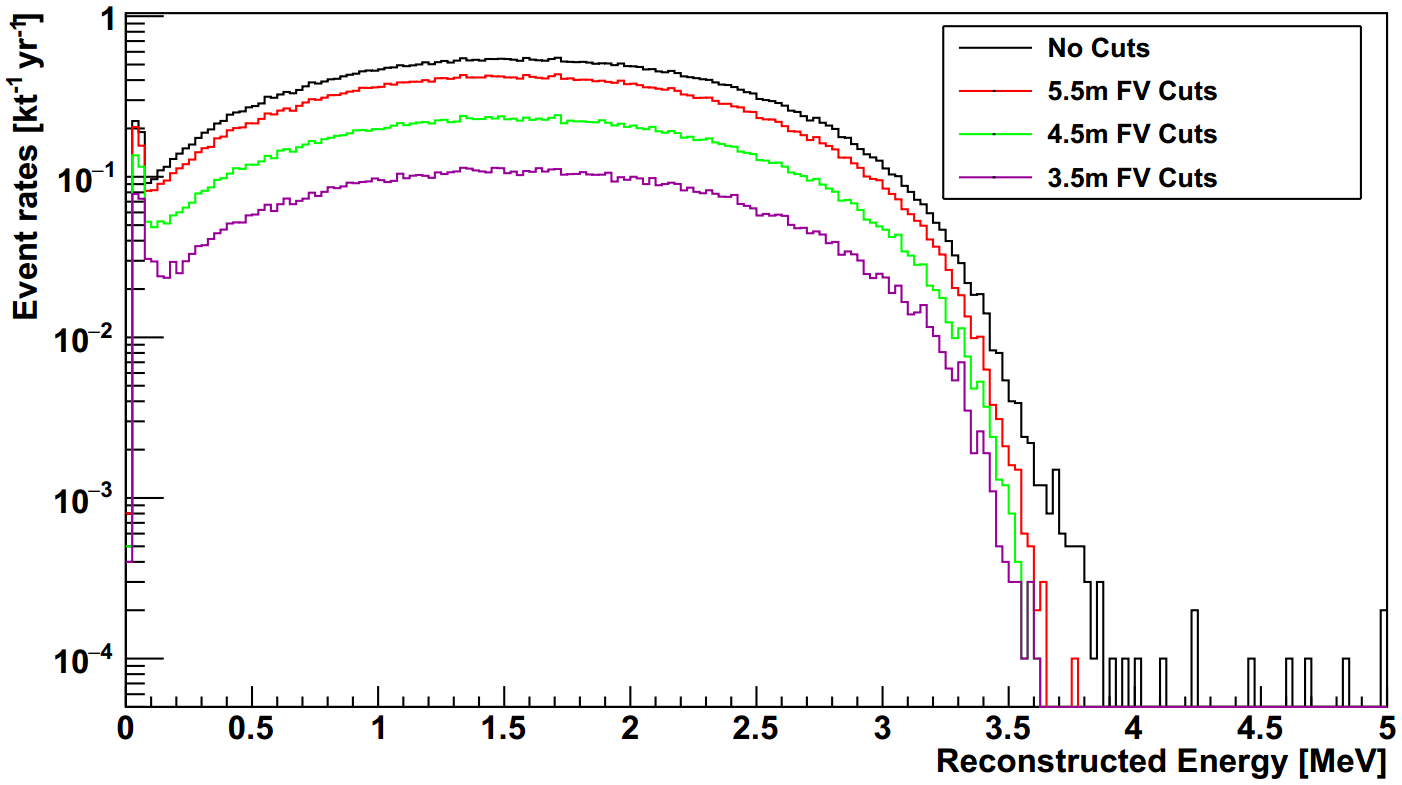
\includegraphics[width=7cm]{muonSolarReconHe6.png}
		\end{minipage}
	}
	\caption{Energy spectrum of cosmic muon induced $^{6}$He backgrounds in SNO+ solar phase for one year duration. Left: Monte Carlo energy distributions. Right: Reconstructed energy distributions.}
	\label{muonSolarHe6}
\end{figure}


\begin{table}[ht]
	\caption{Event rates of cosmic muon induced $^{11}$C, $^{10}$C and $^6$He backgrounds in SNO+ solar phase (unit: $kt^{-1}\cdot yr^{-1}$). FV Cuts ROI [MeV] $^{11}$C events $^{10}$C events $^{6}$He events}
	\centering
	\begin{tabular*}{150mm}{c@{\extracolsep{\fill}}cccccccc}
		\toprule
		\multirow{2}{*}{FV cuts} & \multirow{2}{*}{ROI [MeV]} & \multicolumn{2}{c}{$^{11}$C} & \multicolumn{2}{c}{$^{10}$C} & \multicolumn{2}{c}{$^{6}$He}\\
		\cline{3-4}  \cline{5-6} \cline{7-8}
		&  & MC & Recon.& MC& Recon.& MC& Recon.\\
		\midrule
		No cuts & all regions &  1136.32 & 1107.50 & 24.04& 23.07& 46.99& 45.30\\
		5.5-m & all regions & 862.32& 855.56& 18.20& 17.64& 35.64& 35.25\\
		4.5-m & all regions & 472.12&470.22& 9.92& 9.77& 19.44& 19.41\\
		3.5-m & all regions & 222.05& 221.94& 4.63& 4.66& 9.17& 9.24\\
		\bottomrule		
	\end{tabular*}\label{muon_eventrates2}
\end{table}
